\section{Diseño de la Interfaz de Usuario}

La interfaz de usuario constituye la capa de presentación del sistema y tiene
como propósito poner a disposición del personal del parqueadero la información
generada por el motor de percepción. Su diseño se subordina a tres criterios: la
separación de funciones según el rol del usuario, la prioridad de la información
operativa sobre la información histórica, y la reducción del número de
interacciones necesarias para resolver una incidencia de acceso.

\subsection{Criterios de diseño y estructura de navegación}

La interfaz reconoce tres roles con capacidades diferenciadas. El
\textbf{operador} accede a las vistas de monitoreo, historial e incidentes,
orientadas a la supervisión en tiempo real y a la resolución de incidencias; el
\textbf{administrador} accede además a la gestión de usuarios, al registro de
cámaras, a la consulta estadística y a la administración del padrón de
vehículos habilitados (RF-10); el rol de
\textbf{dueño} (\textit{owner}) accede únicamente a la lectura de ocupación,
historial e indicadores, sin capacidad de modificar registros. Esta
separación responde al principio de menor privilegio, según el cual cada usuario
dispone únicamente de las capacidades necesarias para cumplir su función.

La navegación se organiza de forma plana a partir de un menú principal que se
construye dinámicamente según el rol autenticado, evitando niveles de anidamiento
que dificulten el acceso a las vistas de uso frecuente. La Figura
\ref{fig:navegacion} presenta la estructura de navegación resultante.

Un criterio transversal a todas las vistas es la actualización sin intervención
del usuario. El cliente mantiene un canal persistente con el servicio y recibe
por esa vía las variaciones del estado del recinto, de modo que el panel refleja
un ingreso o una salida en el instante en que el sistema lo consolida, sin
sondeo periódico ni acción manual de refresco. La consulta histórica, en cambio,
se resuelve bajo demanda contra los recursos de la API, ya que su naturaleza no
requiere actualización continua.

\begin{figure}[htbp]
    \centering
    \begin{tikzpicture}
        \spBlock{session}{0,0}{4.0cm}{rosa}
            {Inicio de sesión}{Autenticación del personal}

        \spBlock{menu}{0,-1.9}{5.0cm}{rosa}
            {Menú principal}{Construido según el rol}

        % Bus horizontal de navegación: nivel operativo
        \draw[black!65, line width=0.7pt] (menu.south) -- (0,-3.1);
        \draw[black!65, line width=0.7pt] (-6.9,-3.1) -- (6.9,-3.1);

        \spBlock{vistaMonitoreo}{-5.4,-4.1}{3.0cm}{cielo}
            {Monitoreo}{Tiempo real}
        \spBlock{vistaHistorial}{-1.8,-4.1}{3.0cm}{cielo}
            {Historial}{Eventos}
        \spBlock{vistaIncidentes}{1.8,-4.1}{3.0cm}{cielo}
            {Incidentes}{Discrepancias}
        \spBlock{vistaPadron}{5.4,-4.1}{3.0cm}{purpura}
            {Padrón}{Habilitados}

        % Bus horizontal de navegación: nivel administrativo
        \draw[black!65, line width=0.7pt] (0,-3.1) -- (0,-4.9);
        \draw[black!65, line width=0.7pt] (-6.9,-4.9) -- (6.9,-4.9);

        \spBlock{vistaEstadistica}{-5.4,-5.9}{3.0cm}{purpura}
            {Estadísticas}{Afluencia}
        \spBlock{vistaCamaras}{-1.8,-5.9}{3.0cm}{purpura}
            {Cámaras}{Puntos de acceso}
        \spBlock{vistaUsuarios}{1.8,-5.9}{3.0cm}{purpura}
            {Usuarios}{Roles y cuentas}
        \spBlock{vistaModelo}{5.4,-5.9}{3.0cm}{matblue}
            {Modelo}{Telemetría}

        \foreach \x in {-5.4,-1.8,1.8,5.4} {
            \draw[spflow] (\x,-3.1) -- (\x,-3.62);
            \draw[spflow] (\x,-4.9) -- (\x,-5.42);
        }

    \end{tikzpicture}
    \caption{Estructura de navegación de la aplicación web.}
    \label{fig:navegacion}
\end{figure}

\subsection{Vistas de operación}

Las vistas de operación concentran las funciones de supervisión. La Figura
\ref{fig:wireframes_operacion} presenta sus maquetas esquemáticas. La vista de
monitoreo en tiempo real (Figura \ref{fig:wire_monitoreo}) presenta el flujo de
video del punto de acceso con las cajas delimitadoras superpuestas, el nivel de
ocupación del recinto y, de forma simultánea, el resultado del último evento
procesado: matrícula reconocida, tipo, color y sentido del cruce. Esta
disposición permite al operador verificar en un solo golpe de
vista si la identificación del sistema coincide con lo que observa en la imagen,
y detectar de inmediato una eventual discrepancia entre la ocupación registrada y
la ocupación real.

La vista de historial (Figura \ref{fig:wire_historial}) ofrece una consulta
tabular de los eventos registrados, habilitando filtros por rango de fechas, por
punto de acceso y por matrícula. Cada fila expone la marca temporal, la
matrícula, la cámara de origen, el sentido del cruce y el estado de la sesión, de
modo que el operador pueda localizar y auditar un acceso
específico sin recurrir a la base de datos.

\begin{figure}[htbp]
    \centering

    % ********************** (a) Monitoreo **********************
    \begin{subfigure}[b]{0.48\textwidth}
        \centering
        \begin{tikzpicture}
            \spScreen{wA}{0,0}{7.0}{4.6}{Monitoreo en tiempo real}

            % Panel de video
            \spPanel{-1.85,-0.35}{3.2}{3.6}{Video en vivo}
            \draw[draw=black!40, fill=black!12, line width=0.4pt]
                (-3.25,-1.55) rectangle (-0.45,1.05);

            % Caja delimitadora del vehículo
            \draw[draw=matblue, line width=0.9pt]
                (-2.75,-1.25) rectangle (-1.35,0.05);
            \node[font=\tiny\sffamily, text=matblue!60!black]
                at (-2.05,0.20) {vehículo};

            % Recorte de la placa
            \draw[draw=purpura, fill=yellow!45, line width=0.5pt]
                (-2.55,-0.95) rectangle (-1.55,-0.62);
            \node[font=\tiny\bfseries\sffamily, text=black!75]
                at (-2.05,-0.785) {1234ABC};

            \node[font=\tiny\sffamily, text=black!55]
                at (-1.85,-1.85) {Cámara: ACC-01};

            % Panel del último evento
            \spPanel{1.75,-0.35}{3.4}{3.6}{Último evento}
            \node[anchor=north west, align=left, font=\tiny\sffamily,
                  text=black!75, inner sep=0pt] at (0.20,1.10)
                {Matrícula: \textbf{1234ABC}\\Tipo: Automóvil\\Color: Rojo\\
                 Sentido: Ingreso};

            \draw[black!25, line width=0.4pt] (0.20,-0.10) -- (3.30,-0.10);

            \node[font=\tiny\sffamily, text=black!55] at (1.75,-0.42)
                {Estado de la sesión};
            \spBadge{1.75,-0.78}{green}{REGISTRADO}
            \node[font=\tiny\itshape, text=black!55] at (1.75,-1.30)
                {Sesión creada};

        \end{tikzpicture}
        \caption{Monitoreo en tiempo real.}
        \label{fig:wire_monitoreo}
    \end{subfigure}
    \hfill
    % ********************** (b) Historial **********************
    \begin{subfigure}[b]{0.48\textwidth}
        \centering
        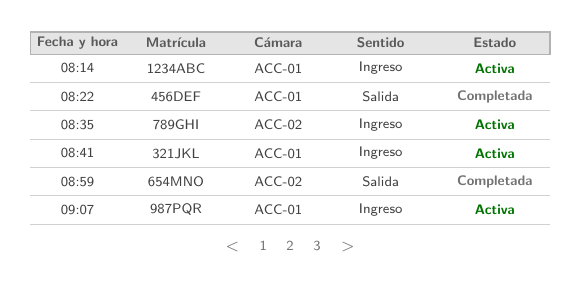
\begin{tikzpicture}
            \spScreen{wB}{0,0}{7.0}{4.6}{Historial de eventos}

            % Barra de filtros
            \spField{-2.45,1.45}{1.3}{Desde: 01/09}
            \spField{-1.05,1.45}{1.3}{Hasta: 30/09}
            \spField{0.45,1.45}{1.4}{Cámara: todas}
            \spField{2.00,1.45}{1.2}{Matrícula}
            \spBadge{3.05,1.45}{cielo}{Buscar}

            % Cabecera de la tabla
            \draw[draw=black!30, fill=black!10, line width=0.4pt]
                (-3.30,0.80) rectangle (3.30,1.08);
            \foreach \x/\t in {-2.70/Fecha y hora, -1.45/Matrícula,
                               -0.15/Cámara, 1.15/Sentido, 2.60/Estado} {
                \node[font=\tiny\bfseries\sffamily, text=black!65]
                    at (\x,0.94) {\t};
            }

            % Filas de datos
            \foreach \y in {0.44,0.08,-0.28,-0.64,-1.00,-1.36} {
                \draw[black!18, line width=0.3pt] (-3.30,\y) -- (3.30,\y);
            }

            \foreach \i/\hora/\placa/\cam/\sen/\est/\col in {%
                1/08:14/1234ABC/ACC-01/Ingreso/Activa/green!45!black,%
                2/08:22/456DEF/ACC-01/Salida/Completada/black!55,%
                3/08:35/789GHI/ACC-02/Ingreso/Activa/green!45!black,%
                4/08:41/321JKL/ACC-01/Ingreso/Activa/green!45!black,%
                5/08:59/654MNO/ACC-02/Salida/Completada/black!55,%
                6/09:07/987PQR/ACC-01/Ingreso/Activa/green!45!black%
            } {
                \node[font=\tiny\sffamily, text=black!75]
                    at (-2.70,{0.98-0.36*\i}) {\hora};
                \node[font=\tiny\sffamily, text=black!75]
                    at (-1.45,{0.98-0.36*\i}) {\placa};
                \node[font=\tiny\sffamily, text=black!75]
                    at (-0.15,{0.98-0.36*\i}) {\cam};
                \node[font=\tiny\sffamily, text=black!75]
                    at (1.15,{0.98-0.36*\i}) {\sen};
                \node[font=\tiny\bfseries\sffamily, text=\col]
                    at (2.60,{0.98-0.36*\i}) {\est};
            }

            \node[font=\tiny\sffamily, text=black!55] at (0,-1.65)
                {\textless{} \quad 1 \quad 2 \quad 3 \quad \textgreater{}};

        \end{tikzpicture}
        \caption{Historial de eventos.}
        \label{fig:wire_historial}
    \end{subfigure}

    \caption{Maquetas de las vistas de operación.}
    \label{fig:wireframes_operacion}
\end{figure}

\subsection{Vistas de administración y análisis}

Las vistas de administración están reservadas al rol de administrador; las de
análisis se ofrecen en modo lectura al administrador y al dueño, y al operador
como apoyo a la operación. La Figura \ref{fig:wireframes_admin} presenta sus
maquetas. La vista de padrón (Figura \ref{fig:wire_padron}) permite registrar,
modificar y desactivar vehículos autorizados, así como auditar su pertenencia al
recinto institucional (RF-10). La vista de estadísticas (Figura
\ref{fig:wire_estadistica}) resume indicadores agregados de la operación
---ingresos y salidas del día y tiempo de permanencia promedio--- y presenta la
distribución de la afluencia por día de la semana, información que sustenta la
toma de decisiones sobre la operación del recinto. La implementación materializó
esta estructura en una vista propia de estadísticas (RF-12), que además alimenta
el panel de monitoreo principal (Figura~\ref{fig:if_panel}), mientras que la
consulta detallada y la exportación residen en el historial de sesiones y el
padrón de vehículos se materializó en una vista administrativa completa
conectada a la detección en tiempo real. La navegación incorporó además la vista
de incidentes y la de telemetría del modelo, y la gestión de usuarios y cámaras,
cuyas maquetas se presentan en la Subsección siguiente y cuya materialización se
documenta con capturas del sistema en operación en el capítulo de implementación.

\begin{figure}[htbp]
    \centering

    % ********************** (c) Padrón **********************
    \begin{subfigure}[b]{0.48\textwidth}
        \centering
        \begin{tikzpicture}
            \spScreen{wC}{0,0}{7.0}{4.6}{Padrón de vehículos}

            \node[anchor=west, font=\tiny\sffamily, text=black!60]
                at (-3.30,1.50) {Vehículos registrados};
            \spBadge{2.35,1.50}{matblue}{+ Nuevo vehículo}

            % Cabecera de la tabla
            \draw[draw=black!30, fill=black!10, line width=0.4pt]
                (-3.30,0.80) rectangle (3.30,1.08);
            \foreach \x/\t in {-2.75/Matrícula, -1.55/Tipo,
                               -0.45/Color, 0.75/Estado, 2.30/Acciones} {
                \node[font=\tiny\bfseries\sffamily, text=black!65]
                    at (\x,0.94) {\t};
            }

            \foreach \y in {0.44,0.08,-0.28,-0.64,-1.00,-1.36} {
                \draw[black!18, line width=0.3pt] (-3.30,\y) -- (3.30,\y);
            }

            \foreach \i/\placa/\tip/\col/\est in {%
                1/1234ABC/Automóvil/Rojo/Activo,%
                2/456DEF/Camioneta/Blanco/Activo,%
                3/789GHI/Minibús/Azul/Activo,%
                4/321JKL/Automóvil/Negro/Inactivo,%
                5/654MNO/Motocicleta/Gris/Activo,%
                6/112PQR/Vagoneta/Plomo/Activo%
            } {
                \node[font=\tiny\sffamily, text=black!75]
                    at (-2.75,{0.98-0.36*\i}) {\placa};
                \node[font=\tiny\sffamily, text=black!75]
                    at (-1.55,{0.98-0.36*\i}) {\tip};
                \node[font=\tiny\sffamily, text=black!75]
                    at (-0.45,{0.98-0.36*\i}) {\col};
                \node[font=\tiny\sffamily, text=black!75]
                    at (0.75,{0.98-0.36*\i}) {\est};
                \node[font=\tiny\sffamily, text=matblue!60!black]
                    at (2.30,{0.98-0.36*\i}) {Editar};
            }

            \node[font=\tiny\sffamily, text=black!55] at (0,-1.62)
                {Mostrando 6 de 42 vehículos registrados};

        \end{tikzpicture}
        \caption{Padrón de vehículos.}
        \label{fig:wire_padron}
    \end{subfigure}
    \hfill
    % ********************** (d) Estadísticas **********************
    \begin{subfigure}[b]{0.48\textwidth}
        \centering
        \begin{tikzpicture}
            \spScreen{wD}{0,0}{7.0}{4.6}{Estadísticas de operación}

            % Tarjetas de indicadores
            \foreach \x/\tit/\val in {-2.35/Ingresos hoy/128,
                                      0/Salidas hoy/115,
                                      2.35/Permanencia/42 min} {
                \draw[draw=black!35, fill=black!4, rounded corners=2pt,
                      line width=0.5pt]
                    (\x-1.05,0.80) rectangle (\x+1.05,1.50);
                \node[font=\tiny\sffamily, text=black!55]
                    at (\x,1.34) {\tit};
                \node[font=\scriptsize\bfseries\sffamily, text=matblue!55!black]
                    at (\x,1.02) {\val};
            }

            % Panel del gráfico de afluencia
            \spPanel{0,-0.85}{6.6}{2.4}{Afluencia por día de la semana}

            \draw[black!45, line width=0.6pt] (-3.05,-1.75) -- (3.05,-1.75);

            \foreach \i/\lab/\val in {1/Lu/85,2/Ma/80,3/Mi/96,
                                       4/Ju/76,5/Vi/66,6/Sá/96} {
                \pgfmathsetmacro{\bh}{\val/96*1.5}
                \draw[draw=matblue!70!black, fill=matblue!35, line width=0.4pt]
                    ({-2.40+(\i-1)*0.96-0.32},-1.75)
                    rectangle ({-2.40+(\i-1)*0.96+0.32},{-1.75+\bh});
                \node[font=\tiny\sffamily, text=black!60]
                    at ({-2.40+(\i-1)*0.96},-1.92) {\lab};
            }

        \end{tikzpicture}
        \caption{Estadísticas de operación.}
        \label{fig:wire_estadistica}
    \end{subfigure}

    \caption{Maquetas de las vistas de administración y análisis.}
    \label{fig:wireframes_admin}
\end{figure}

\subsection{Vistas de incidencia y diagnóstico}

El sistema reconoce que el reconocimiento automático de matrículas es
probabilístico y que, bajo las condiciones de captura del entorno de estudio,
una fracción de las salidas no encontrará coincidencia exacta con una sesión
activa. Por esa razón, la interfaz incorpora una vista específica de incidencias
(Figura \ref{fig:wire_incidentes}) cuyo propósito es resolver la discrepancia en
el menor número de interacciones posible. La vista presenta, a la izquierda, la
lista de discrepancias pendientes con la matrícula leída, su confianza y la hora;
y a la derecha, el detalle de la incidencia seleccionada con los fotogramas de
ingreso y salida, la lista de sesiones candidatas ordenadas por aproximación
temporal y la acción de cierre manual, que queda registrada con el operador y el
motivo.

La vista de telemetría del modelo (Figura \ref{fig:wire_modelo}) completa el
conjunto. Está destinada al administrador y al responsable técnico: expone la
latencia de inferencia por fotograma, los indicadores agregados de desempeño y la
versión del modelo en operación, de modo que una degradación del servicio pueda
atribuirse a la captura, a la red o al motor de percepción sin acceso directo a
la base de datos.

\begin{figure}[H]
    \centering

    % ********************** (e) Incidentes **********************
    \begin{subfigure}[b]{0.48\textwidth}
        \centering
        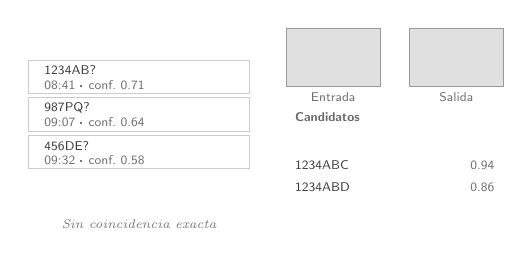
\begin{tikzpicture}[scale=0.92, every node/.style={transform shape}]
            \spScreen{wE}{0,0}{7.0}{4.6}{Incidencias de acceso}

            % Lista de incidencias
            \spPanel{-1.75,0.05}{3.3}{3.3}{Pendientes (3)}
            \foreach \i/\hora/\placa/\conf in {%
                1/08:41/1234AB?/{0.71},%
                2/09:07/987PQ?/{0.64},%
                3/09:32/456DE?/{0.58}%
            } {
                \pgfmathsetmacro{\yc}{1.20-0.52*\i}
                \draw[draw=black!20, fill=white, line width=0.4pt]
                    (-3.28,{\yc-0.23}) rectangle (-0.22,{\yc+0.23});
                \node[anchor=west, font=\tiny\sffamily, text=black!75]
                    at (-3.18,{\yc+0.09}) {\placa};
                \node[anchor=west, font=\tiny\sffamily, text=black!55]
                    at (-3.18,{\yc-0.11}) {\hora\ \textperiodcentered\ conf.\ \conf};
            }
            \node[font=\tiny\itshape, text=black!55] at (-1.75,-1.35)
                {Sin coincidencia exacta};

            % Detalle de la incidencia
            \spPanel{1.75,0.05}{3.3}{3.3}{Detalle seleccionado}

            \draw[draw=black!40, fill=black!12, line width=0.4pt]
                (0.28,0.55) rectangle (1.58,1.35);
            \node[font=\tiny\sffamily, text=black!55] at (0.93,0.40) {Entrada};

            \draw[draw=black!40, fill=black!12, line width=0.4pt]
                (1.98,0.55) rectangle (3.28,1.35);
            \node[font=\tiny\sffamily, text=black!55] at (2.63,0.40) {Salida};

            \node[anchor=west, font=\tiny\bfseries\sffamily, text=black!60]
                at (0.28,0.12) {Candidatos};
            \foreach \i/\placa/\conf in {1/1234ABC/{0.94}, 2/1234ABD/{0.86}} {
                \pgfmathsetmacro{\yc}{-0.24-0.30*\i}
                \node[anchor=west, font=\tiny\sffamily, text=black!75]
                    at (0.28,\yc) {\placa};
                \node[anchor=east, font=\tiny\sffamily, text=black!55]
                    at (3.28,\yc) {\conf};
            }
            \spBadge{1.75,-1.30}{green}{Cerrar sesión}

        \end{tikzpicture}
        \caption{Incidencias de acceso y cierre asistido.}
        \label{fig:wire_incidentes}
    \end{subfigure}
    \hfill
    % ********************** (f) Telemetría del modelo **********************
    \begin{subfigure}[b]{0.48\textwidth}
        \centering
        \begin{tikzpicture}[scale=0.92, every node/.style={transform shape}]
            \spScreen{wF}{0,0}{7.0}{4.6}{Telemetría del modelo}

            % Tarjetas de indicadores
            \foreach \x/\tit/\val in {-2.35/Latencia/38 ms,
                                      0/FPS/{12.4},
                                      2.35/Versión/yolo26n} {
                \draw[draw=black!35, fill=black!4, rounded corners=2pt,
                      line width=0.5pt]
                    (\x-1.05,0.80) rectangle (\x+1.05,1.50);
                \node[font=\tiny\sffamily, text=black!55]
                    at (\x,1.34) {\tit};
                \node[font=\scriptsize\bfseries\sffamily, text=matblue!55!black]
                    at (\x,1.02) {\val};
            }

            % Panel de latencia por fotograma
            \spPanel{-1.75,-0.85}{3.3}{2.4}{Latencia por fotograma}
            \draw[black!45, line width=0.5pt] (-3.30,-1.80) -- (-0.25,-1.80);
            \draw[draw=matblue, line width=0.8pt]
                (-3.20,-1.20) -- (-2.85,-1.05) -- (-2.50,-1.25) --
                (-2.15,-0.98) -- (-1.80,-1.10) -- (-1.45,-1.32) --
                (-1.10,-1.08) -- (-0.75,-1.18) -- (-0.40,-1.02);

            % Panel de estado de componentes
            \spPanel{1.75,-0.85}{3.3}{2.4}{Estado de componentes}
            \foreach \i/\comp/\est/\col in {%
                1/Captura/En l\'inea/green,%
                2/Inferencia/En l\'inea/green,%
                3/Base de datos/En l\'inea/green,%
                4/Cola/1 tarea/black%
            } {
                \node[anchor=west, font=\tiny\sffamily, text=black!70]
                    at (0.25,{-0.05-0.42*\i}) {\comp};
                \node[anchor=east, font=\tiny\bfseries\sffamily, text=\col!55!black]
                    at (3.25,{-0.05-0.42*\i}) {\est};
            }

        \end{tikzpicture}
        \caption{Telemetría del modelo y estado de componentes.}
        \label{fig:wire_modelo}
    \end{subfigure}

    \caption{Maquetas de las vistas de incidencia y diagnóstico.}
    \label{fig:wireframes_diagnostico}
\end{figure}
